\chapter{Training of the CNN}
\label{ch:training_of_the_cnn}

Building a \acrlong{cnn} from scratch leaves a lot of design choices and requires multiple steps.
The first step involves the design of the desired \acrshort{cnn} architecture.
In a second step, the labeled dataset is used to fit the \acrshort{cnn} model.
If necessary, the hyperparameters of the \acrshort{cnn} architecture can be tuned in a third step.

This chapter describes the dataset generation, the design of the \acrshort{cnn} architecture and the actual training of the \acrshort{cnn} model.

\section{Dataset}
\label{sec:training_of_the_cnn:dataset}

The dataset contains frames of 22 different throwing objects, as shown in table \ref{tab:objects}.
It is fully labeled and consists of more than \num{15000} usable frames with at least \num{485} frames of each object.
All frames were collected over the course of two days during the previous project.
Figure \ref{fig:dataset} shows two example frames from the dataset (the \textit{Stuffed Bunny} and the \textit{Hand Featherball}).

\begin{table}
  \caption{List of the different throwing objects}
  \label{tab:objects}
  \centering
  \begin{tabular}{llll}
    \toprule
    \textbf{Objects} &  &  &  \\
    \midrule
    Nerf Dart & American Football & Table Tennis Ball & Shuttlecock \\ % left to right, top to bottom
    Sporf & Arrow & Hand Featherball & Floorball \\
    Spiky Ball & Tesafilm & Sponge & Red Duplo Brick \\
    Green Duplo Brick & Duplo Figure & Foam Die & Infant Shoe \\
    Stuffed Bunny & Goalkeeper Glove & Hemp Cord & Paper Ball \\
    Beer Cap & Water Bottle &  &  \\
    \bottomrule
  \end{tabular}
\end{table}

\begin{figure}[t]
  \centering
  \begin{subfigure}[b]{0.45\textwidth}
    \centering
    \includegraphics[width=\textwidth]{1574952009_278_10_stuffed-bunny}
    \caption{Stuffed Bunny}
    \label{subfig:dataset_stuffed_bunny}
  \end{subfigure}
  \begin{subfigure}[b]{0.45\textwidth}
    \centering
    \includegraphics[width=\textwidth]{1574943825_125_8_hand-featherball}
    \caption{Hand Featherball}
    \label{subfig:dataset_hand_featherball}
  \end{subfigure}
  \caption{Two example frames from the dataset}
  \label{fig:dataset}
\end{figure}

% ------------------------------------------------------------------------------------------------------------------------------
\subsection{White Balance}
\label{subsec:training_of_the_cnn:dataset:white_balance}

A notable thing is that on the first day of the data collection, the white balance was performed continuously (every three frames).
This caused the background color of large colored objects to be distorted, as shown in figure \ref{fig:white_balance}.
However, this is not problematic, as noise can improve the generalization and thus reduce overfitting \cite{training_noise}.

\begin{figure}[t]
  \centering
  \begin{subfigure}[b]{0.45\textwidth}
    \centering
    \includegraphics[width=\textwidth]{1574950250_238_9_foam-dice}
    \caption{Continuous white balance}
    \label{subfig:white_balance_first_day}
  \end{subfigure}
  \begin{subfigure}[b]{0.45\textwidth}
    \centering
    \includegraphics[width=\textwidth]{1575032343_726_8_foam-dice}
    \caption{One-off white balance}
    \label{subfig:white_balance_second_day}
  \end{subfigure}
  \caption{White balance difference between the first (\subref{subfig:white_balance_first_day}) and the second (\subref{subfig:white_balance_second_day}) day}
  \label{fig:white_balance}
\end{figure}

% ------------------------------------------------------------------------------------------------------------------------------
\subsection{Statistics}
\label{subsec:training_of_the_cnn:dataset:statistics}

Figure \ref{fig:statistics} shows the amount of captured frames for each object individually.
It is evident that there are generally more frames of larger objects.
This is, on the one hand, due to the specific implementation of the throw detection mechanism.
On the other hand, the field of view of the camera is not uniformly illuminated (the center is brighter than the edges).
For those reasons, a larger object area is required at the borders to achieve a sufficiently large change in the frame.
However, this also leads to the fact that larger objects are more often only partially in the frame.

The statistics of the dataset reveal that it is slightly imbalanced.
This fact has to be taken into account when creating the various dataset splits (see section \ref{subsec:training_of_the_cnn:dataset:splitting}) that are required for the fitting and evaluation of the model.

An imbalanced dataset can lead to serious problems, e.g. a bias towards the classes with the most samples.
Consider a dataset consisting of only two classes that is imbalanced in such a way that \SI{90}{\percent} of all samples belong to class \texttt{A}.
The fitting process of the classification model will naturally favor class \texttt{A}, since the chance of being right is nine times higher.
The classification could even be independent of the input and always opt for class \texttt{A} (completely ignoring class \texttt{B}).
This obviously terrible classification process would still result in an overall accuracy of \SI{90}{\percent} \cite{training_imbalanced}.

\begin{figure}
  \centering
  \includegraphics[width=\textwidth]{statistics}
  \caption{Statistics showing the amount of captured frames for each object individually}
  \label{fig:statistics}
\end{figure}

% ------------------------------------------------------------------------------------------------------------------------------
\subsection{Augmentation}
\label{subsec:training_of_the_cnn:dataset:augmentation}

The image dimensions of the individual frames are $1280\times\SI{1024}{px}$ (width $\times$ height) with three color channels (\acrshort{rgb}).
This is an enormous amount of input data for a \acrlong{cnn} and would result in an extremely large amount of mathematical operations to classify even a single frame.
As a result, the classification throughput is reduced and thus the time required to fit the \acrshort{cnn} model is greatly increased.

Another important aspect of the dataset is the fact that it was collected over the course of only two days.
Some objects (e.g. the \textit{Water Bottle}) were even added only on the second day of the data collection.
Real-world observations have shown that the surrounding ambient light and the orientation of an object have a significant influence on the classification performance.
The data collection took place in a relatively dim location and the ambient light did not change much.
The classification performance is therefore much better when there is less ambient light.

Furthermore, the orientation of an object on a frame also impacts the classification performance.
One such problem arises if, for example, the \textit{Shuttlecock} is deliberately thrown with the plastic tail feathers in front of the cork head.
Experiments have shown that this results in a complete misclassification of the object.

For those reasons, a range of image data augmentation techniques are used on the individual frames to improve the real-world classification performance \cite{training_data_augmentation}.
The dataset augmentation is done with the Python script \texttt{dataset\_generator.py}, which uses NumPy as well as the Python implementation of the \acrfull{opencv}.
NumPy provides support for large, multi-dimensional arrays and an assortment of functions to work on these arrays \cite{training_numpy}.
\acrshort{opencv} provides various image transformation functions (e.g. resizing, color space conversions) and conveniently uses NumPy arrays to represent the images \cite{training_opencv_intro}.

% -----------------------
\paragraph{Image Scaling}
To reduce the input data of the \acrshort{cnn} model, the width and height of the individual frames are each scaled down by a factor of four.
This results in an image with the dimensions of $320\times\SI{256}{px}$ (width $\times$ height) and thus in a data reduction of \num{16}.

These dimensions are great because even the important features of the smallest objects are still preserved.
Given that the background of the frames remains more or less the same, a reasonably deep \acrshort{cnn} should have no problems distinguishing between the only \num{22} different classes.

The downsampling is achieved with the use of nearest-neighbor interpolation.
This results in more noise and scaling artifacts than other interpolation methods, such as bilinear or bicubic interpolation.
The scaling artifacts shown in figure \ref{fig:augmentation_downsampling} are the result of aliasing.
The advantages of nearest-neighbor interpolation are its simplicity and fast execution time \cite{training_interpolation}.
Furthermore, the additional noise can improve the generalization and therefore reduce overfitting \cite{training_noise}.

The Python implementation of the image scaling makes use of the \acrshort{opencv} function \texttt{cv2.resize}.
This function is supplied with three arguments: the NumPy array that represents the image, the desired output image size and the interpolation method \cite{training_opencv_resize}.

\begin{figure}
  \centering
  \begin{subfigure}[b]{0.45\textwidth}
    \centering
    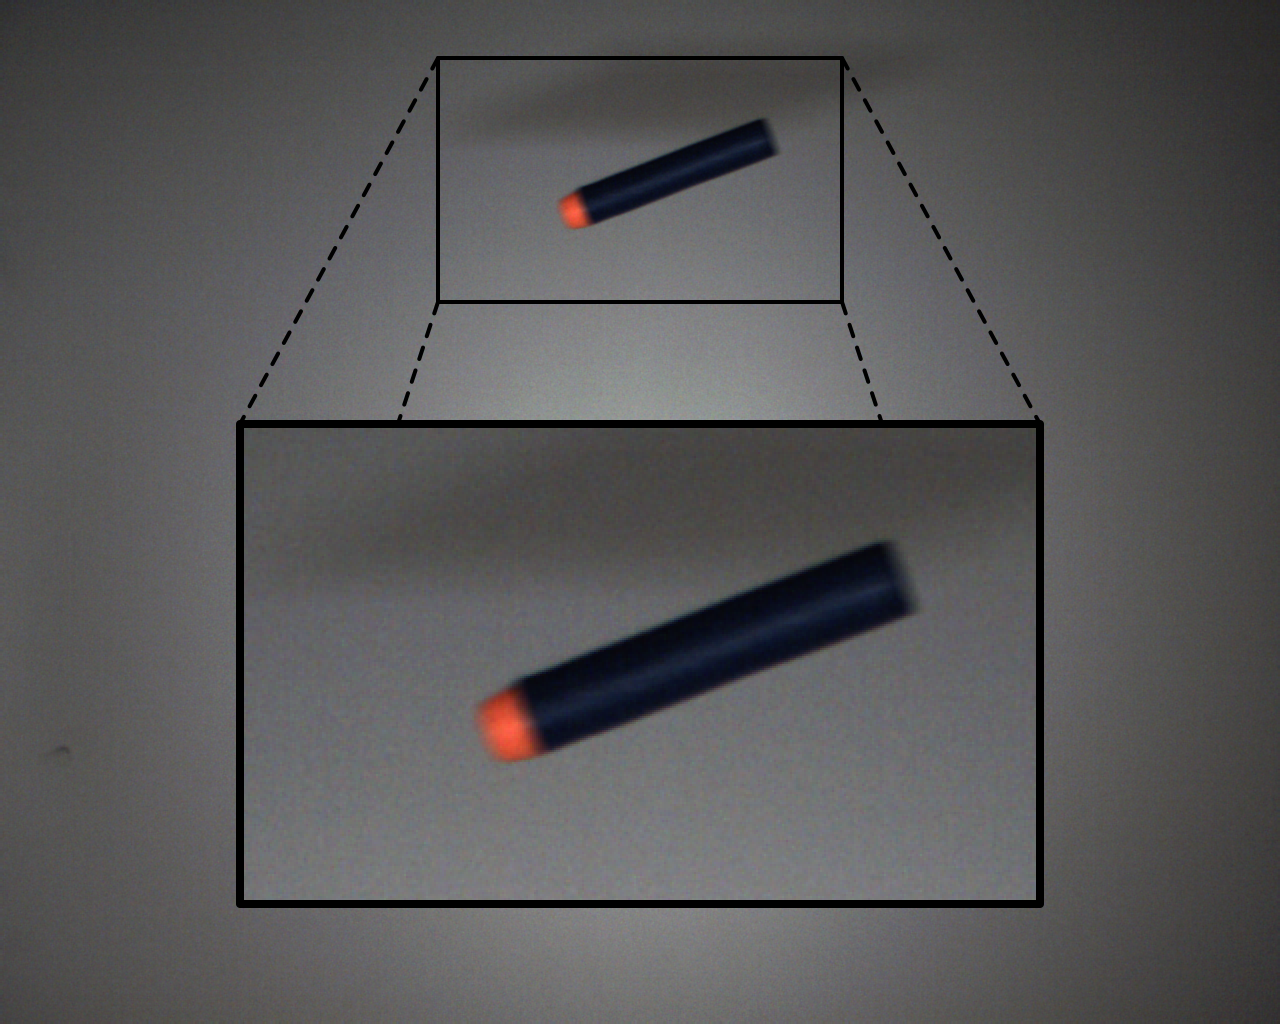
\includegraphics[width=\textwidth]{augmentation_downsampling/1575032863_742_3_nerf-dart_zoom}
    \caption{Original version}
    \label{subfig:ad_original}
  \end{subfigure}
  \begin{subfigure}[b]{0.45\textwidth}
    \centering
    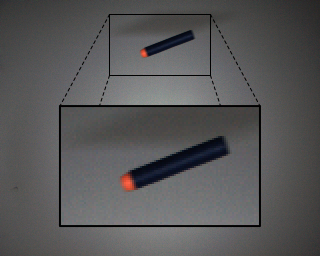
\includegraphics[width=\textwidth]{augmentation_downsampling/1575032863_742_3_nerf-dart_resized_zoom}
    \caption{Scaled-down version}
    \label{subfig:ad_resized}
  \end{subfigure}
  \caption{Example of an original (\subref{subfig:ad_original}) and a scaled-down version (\subref{subfig:ad_resized}) of a frame ($2\times$ inner zoom added to better highlight the difference)}
  \label{fig:augmentation_downsampling}
\end{figure}

% ---------------------
\paragraph{Color Space}
To reduce the dependence on ambient light intensity, the average brightness of the individual frames is changed.
The rounded average brightness $B$ of an image can be calculated using equation \ref{eq:rounded_average_brightness}.
This equation is implemented in Python with the help of the NumPy function \texttt{np.sum}, which computes the sum of all array elements \cite{training_numpy_sum}.

\begin{equation}
  B = \left\lfloor\frac{1}{w\cdot h\cdot c} \cdot \sum\limits_{k=1}^c \sum\limits_{i=1}^h \sum\limits_{j=1}^w \boldsymbol{M}_{ij}^{k} + 0.5\right\rfloor
  \label{eq:rounded_average_brightness}
\end{equation}

where

\begin{tabular}{lll}
  $B$ & = & rounded average brightness \\
  $w$ & = & width of the image \\
  $h$ & = & height of the image \\
  $c$ & = & number of channels \\
  $\boldsymbol{M}^k$ & = & pixel matrix of channel $k$ \\
\end{tabular}
\\

\clearpage

The rounded average brightness of the background was computed at various times of the day and lies between \numrange{85}{160}.
This range includes environments without ambient light as well as environments with indirect sunlight and artificial ambient light.
In the light of these results, a step size of \num{15} was chosen to cover this spectrum of ambient light intensities.
This results in the following six discrete average brightness levels: \num{85}, \num{100}, \num{115}, \num{130}, \num{145} and \num{160}.

Calculating the average brightness of the individual frames is problematic, as the frames contain objects in addition to the background.
For this reason, only the first frame of a throw (which presumably consists mainly of background) is used to compute the average brightness $B_1$.
This value is then used to determine the required brightness offset $\Delta$ for all frames of that throw as shown in equation \ref{eq:offset_calculation}.

\begin{equation}
  \Delta = B_{\text{des}} - B_1
  \label{eq:offset_calculation}
\end{equation}

where

\begin{tabular}{lll}
  $\Delta$ & = & required brightness offset \\
  $B_{\text{des}}$ & = & desired, rounded average brightness \\
  $B_1$ & = & rounded average brightness of the first frame of the throw \\
\end{tabular}
\\

The brightness adjustment is done according to equation \ref{eq:brightness_adjustment}.
The implementation of this equation in Python consists of two steps.
In a first step, the required brightness offset $\Delta$ is added to each pixel of each color channel individually.
The pixel values are 8-bit unsigned integers, which must be in the range between \numrange{0}{255}.
In order to ensure that this range is not exceeded, the values are clipped in a second step.
For this purpose, the NumPy function \texttt{np.clip} is used \cite{training_numpy_clip}.

\begin{equation}
  A_{i,j}^{k} =
  \begin{cases}
    0 & M_{i,j}^{k} + \Delta < 0 \\
    M_{i,j}^{k} + \Delta & 0\leq M_{i,j}^{k} + \Delta\leq 255 \\
    255 & M_{i,j}^{k} + \Delta > 255 \\
  \end{cases}
  \label{eq:brightness_adjustment}
\end{equation}

where

\[
  i = 1, 2, \dots, h \quad \text{and} \quad j = 1, 2, \dots, w \quad \text{and} \quad k = 1, 2, \dots, c
\]

and

\begin{tabular}{lll}
  $A_{i,j}^{k}$ & = & element $i,j$ of the $k$-th channel augmented pixel matrix $\boldsymbol{A}$ \\
  $M_{i,j}^{k}$ & = & element $i,j$ of the $k$-th channel pixel matrix $\boldsymbol{M}$ \\
  $\Delta$ & = & required brightness offset \\
  $h$ & = & height of the image \\
  $w$ & = & width of the image \\
  $c$ & = & number of channels \\
\end{tabular}
\\

Figure \ref{fig:augmentation_brightness} shows an example of the resized frames of the \textit{Water Bottle}, where the brightness levels were adjusted.
For this example, frame \num{12} of throw \num{575} was used.
The rounded average brightness of the first frame of this throw $B_1$ is equal to \num{101}, whereas $B_{12}$ is equal to \num{99}.
Therefore, an additional offset of \num{-2} in regard to the desired brightness levels is expected.
This is due to the fact that the required brightness offset is determined by using the rounded average brightness of the first frame rather than the frame that is being adjusted.

\begin{figure}
  \centering
  \begin{subfigure}[b]{0.15\textwidth}
    \centering
    \includegraphics[width=\textwidth]{augmentation_brightness/1575026107_575_12_water-bottle_85}
    \caption{$B = 83$}
    \label{subfig:ab_85}
  \end{subfigure}
  \begin{subfigure}[b]{0.15\textwidth}
    \centering
    \includegraphics[width=\textwidth]{augmentation_brightness/1575026107_575_12_water-bottle_100}
    \caption{$B = 98$}
    \label{subfig:ab_100}
  \end{subfigure}
  \begin{subfigure}[b]{0.15\textwidth}
    \centering
    \includegraphics[width=\textwidth]{augmentation_brightness/1575026107_575_12_water-bottle_115}
    \caption{$B = 113$}
    \label{subfig:ab_115}
  \end{subfigure}
  \begin{subfigure}[b]{0.15\textwidth}
    \centering
    \includegraphics[width=\textwidth]{augmentation_brightness/1575026107_575_12_water-bottle_130}
    \caption{$B = 128$}
    \label{subfig:ab_130}
  \end{subfigure}
  \begin{subfigure}[b]{0.15\textwidth}
    \centering
    \includegraphics[width=\textwidth]{augmentation_brightness/1575026107_575_12_water-bottle_145}
    \caption{$B = 143$}
    \label{subfig:ab_145}
  \end{subfigure}
  \begin{subfigure}[b]{0.15\textwidth}
    \centering
    \includegraphics[width=\textwidth]{augmentation_brightness/1575026107_575_12_water-bottle_160}
    \caption{$B = 158$}
    \label{subfig:ab_160}
  \end{subfigure}
  \caption{Examples of resized frames of the \textit{Water Bottle}, where the brightness was adjusted according to the desired brightness levels}
  \label{fig:augmentation_brightness}
\end{figure}

% ------------------
\paragraph{Flipping}
Each frame is flipped vertically and horizontally to improve the orientation-independence of the objects in the frames.
Furthermore, the influence of the shadow that the object casts is decreased.
An example of these reflections is shown in figure \ref{fig:augmentation_flipping}.

The Python implementation uses the \acrshort{opencv} function \texttt{cv2.flip} to flip the frames around the x-axis (vertically) and around the y-axis (horizontally) \cite{training_opencv_flip}.

\begin{figure}
  \centering
  \begin{subfigure}[b]{0.3\textwidth}
    \centering
    \includegraphics[width=\textwidth]{augmentation_flipping/1575023302_468_9_shuttlecock}
    \caption{Unaugmented}
    \label{subfig:af_resized}
  \end{subfigure}
  \begin{subfigure}[b]{0.3\textwidth}
    \centering
    \includegraphics[width=\textwidth]{augmentation_flipping/1575023302_468_9_shuttlecock_v}
    \caption{Vertically flipped}
    \label{subfig:af_vertical}
  \end{subfigure}
  \begin{subfigure}[b]{0.3\textwidth}
    \centering
    \includegraphics[width=\textwidth]{augmentation_flipping/1575023302_468_9_shuttlecock_h}
    \caption{Horizontally flipped}
    \label{subfig:af_horizontal}
  \end{subfigure}
  \caption{Example of a resized frame of the \textit{Shuttlecock} (\subref{subfig:af_resized}), which was flipped vertically (\subref{subfig:af_vertical}) and horizontally (\subref{subfig:af_horizontal})}
  \label{fig:augmentation_flipping}
\end{figure}

% ------------------------------------------------------------------------------------------------------------------------------
\subsection{Splitting}
\label{subsec:training_of_the_cnn:dataset:splitting}
During the fitting and evaluation process of the \acrshort{cnn} model, three splits of the dataset are required.
These required splits and their respective use is summarized in table \ref{tab:dataset_splits}.

\begin{table}
  \caption{Overview of the required dataset splits \cite{training_datasets}}
  \label{tab:dataset_splits}
  \centering
  \begin{tabular}{llp{10cm}}
    \toprule
    \textbf{Dataset} & \textbf{Split} & \textbf{Description} \\
    \midrule
    \textbf{Training} & \SI{70}{\percent} & The training split is used to fit the model. \\
    \midrule
    \textbf{Validation} & \SI{15}{\percent} & The validation split provides an evaluation of a model fit while tuning hyperparameters of the model. \\
    \midrule
    \textbf{Test} & \SI{15}{\percent} & The test split provides an unbiased evaluation of the final model fit (used to compare fit with other final models). \\
    \bottomrule
  \end{tabular}
\end{table}

It is crucial that the dataset splits are used in the right way.
For example, the validation and the test splits must never be used to fit the model.
Furthermore, it is important to know that the evaluation with the validation split becomes more biased as the classification performance is increased by tuning the hyperparameters of the model.
For this reason, a test split is used to evaluate and compare the final model fit.

The quantization process requires a small unlabeled dataset consisting of \numrange{100}{1000} frames for the calibration of the quantized model.
Seeing that the calibration of the quantized model has many similarities to the tuning of the hyperparameters, the required frames are chosen at random from the validation split.
In total, \num{990} frames are chosen from the validation split (largest possible multiple of the \num{22} classes).
The calibration dataset is thus a subset of the validation dataset without labels.

% ------------------------
\paragraph{Implementation}
The splitting of the dataset is implemented in the Python script \texttt{dataset\_generator.py}, which uses NumPy, \acrshort{opencv} and the standard library.

In a first step, the necessary information about the dataset is fetched from the \acrshort{mysql} database, which is used to store the labels, the file names and other useful metadata.
Table \ref{tab:tab_frames_structure} lists all columns of the database table \texttt{aionfpga.frames}.

\begin{table}
  \caption{Structure of the \acrshort{mysql} database table \texttt{aionfpga.frames}}
  \label{tab:tab_frames_structure}
  \centering
  \begin{tabular}{llll}
    \toprule
    \textbf{Column} & \textbf{Type} & \textbf{Length} & \textbf{Description} \\
    \midrule
    id & \texttt{INT} &  & Sequence number (unique identifier) \\
    timestamp & \texttt{INT} &  & The Unix timestamp at the time of the throw \\
    throwid & \texttt{INT} &  & Throw sequence number \\
    frameid & \texttt{INT} &  & Frame sequence number within a throw \\
    frame & \texttt{VARCHAR} & 255 & The file name of the frame \\
    object & \texttt{VARCHAR} & 255 & The name of the object in the frame (label) \\
    framegood & \texttt{INT} &  & \texttt{0}: frame unusable | \texttt{1}: frame usable \\
    partial & \texttt{INT} &  & \texttt{0}: object fully visible | \texttt{1}: object partially visible \\
    \bottomrule
  \end{tabular}
\end{table}

The slight imbalance in the dataset is mitigated in a next step.
There are several different methods to ensure that the dataset is balanced (e.g. collecting more data, resampling).
For the sake of simplicity, undersampling is used to remove samples from the overrepresented classes \cite{training_imbalanced}.

The actual implementation randomly selects frames from each class.
The number of selected frames is equal to the number of frames in the minority class.
The pseudorandom function used for the selection process is seeded to ensure repeatable results during different tests.
In this case, this results in a loss of about \SI{30.9}{\percent} of the collected frames.

In a third step, the data augmentation discussed in section \ref{subsec:training_of_the_cnn:dataset:augmentation} is performed.
The frames are first resized, then their brightness is adjusted and lastly they are flipped.
The brightness adjustment increases the size of the dataset by a factor of seven and the flipping by a factor of three.
This is due to the fact, that the original frames are preserved as well and results in a total increase of the dataset size by a factor of \num{21}.
Original refers in this case to the resized frames.

The next step is the actual splitting of the dataset.
For this purpose, the entire dataset is shuffled and then split according to table \ref{tab:dataset_splits}.

In a last step, the frames and the labels of the dataset splits are separately saved to the disk.
Due to the sheer number of frames in the dataset splits, the frames are saved in batches of \num{32}.
For this reason, \num{32} frames at a time are stored in a four-dimensional NumPy array of type \texttt{np.uint8} with a shape of $32\times 256\times 320\times 3$ (batch size $\times$ height $\times$ width $\times$ number of color channels).
The \num{22} different labels of the classes (object names) are mapped to a unique number between \num{0} and \num{21}.
This allows for an efficient way to store the labels in one-dimensional NumPy arrays of type \texttt{np.uint8}.
The length of these label arrays is determined by the number of frames in the respective splits.

For each split, both the batch arrays and the label array are saved to the disk in the binary NumPy (\texttt{.npy}) file format \cite{training_numpy_format}.
This allows for fast loading of the dataset from the disk \cite{training_numpy_npy}.

Listing \ref{lst:save_batches} shows the function \texttt{save\_batches}, which implements this last step.

\begin{lstlisting}[style=python, caption={Python function \texttt{save\_batches} to save the batch arrays and the label array}, label=lst:save_batches]
def save_batches(frames_name, labels_name, dst, frame_names, batch_size):

  num_frames = len(frame_names)
  num_batches = math.ceil(num_frames / batch_size)

  labels = np.empty((num_frames,), dtype=np.uint8)
  for idx in range(num_batches):
    start = idx * batch_size
    end = start + batch_size
    frame_names_slice = frame_names[start:end]

    frames = np.empty((len(frame_names_slice),) + fh.inf_shape, dtype=np.uint8)
    for i, frame in enumerate(frame_names_slice):
      obj_san = frame.split('_')[3]
      label = fh.objects_san.index(obj_san)
      frames[i] = cv2.imread(str(fh.dir_frames_augmented / f'{frame}.png'))
      labels[idx * batch_size + i] = label

    np.save(dst / f'{frames_name}_batch_{idx}_of_{num_batches}.npy', frames)

  np.save(dst / f'{labels_name}.npy', labels)
\end{lstlisting}

% ----------------
\paragraph{Result}
The toal number of frames after the augmentation is equal to \num{224070}.
The final training dataset consists of \num{156882} frames and requires \SI{35.91}{GiB} of disk space.
The validation and test datasets each comprise of \num{33594} frames and require \SI{15.38}{GiB} of disk space together.

\section{Architecture}
\label{sec:training_of_the_cnn:architecture}

Designing a \acrlong{cnn} architecture from scratch requires choosing the types of layers and their arrangement as well as many hyperparameters.
For this reason, a lot of trial an error is involved in the design process of an adequate model \cite{training_arch_design}.
There are, however, certain design principles that work really well \cite{training_arch_hyper}:

\begin{enumerate}
  \item Starting with a low number of filters (high-level feature detection)
  \item Increasing the number of filters towards the end (low-level feature detection)
  \item Decreasing the spatial dimensions of the feature maps towards the end
  \item Using kernel sizes of $3\times 3$, $5\times 5$ or $7\times 7$ for convolutional layers
  \item Using pool sizes of $2\times 2$ or $3\times 3$ with a stride of two for max-pooling layers
  \item Adding additional layers until the model is overfitting
  \item Using state-of-the-art networks as inspiration
\end{enumerate}

A summary of all the layers of the final \acrshort{cnn} architecture is listed in table \ref{tab:arch}.
The first convolutional layer uses only \num{16} filters and a larger kernel size of $5\times 5$ due to the large dimensions of the input images.
All other convolutional layers use a kernel size of $3\times 3$ while steadily increasing the number of used filters up to \num{128}.
The designed architecture uses six max-pooling layers with a pool size of $2\times 2$ and a stride of two.
This reduces the spatial dimensions of the feature maps to $4\times 5$ (height $\times$ width).
The output of the fully-connected layer \texttt{fc8} is about the size of the output layer \texttt{fc9} squared.
This allows the output layer to combine many of the different high-level features to create a confident prediction.

Even though the model was not yet overfitting, no additional layers were added.
The reason for this is that with the current architecture the classification performance is already exceptional.

Furthermore, the number of trainable parameters (weights) is relative low compared to state-of-the-art networks like VGG, ResNet or Inception \cite{training_arch_keras}.
This increases the throughput considerably, as less mathematical operations are required.
The key to keeping the total number of trainable parameter low is evident when analyzing table \ref{tab:arch}.
A whopping \num{1311232} of the \num{1614486} total weights can be attributed to the connection between the feature maps of the last convolutional layer \texttt{conv7} and the artificial output neurons of the first dense layer \texttt{fc8}.
This accounts for \SI{81.22}{\percent} of all trainable parameters.
For this reason the spatial dimensions of the feature maps should be decreased towards the end.

\begin{table}
  \caption{Layers of the \acrshort{cnn} architecture}
  \label{tab:arch}
  \centering
  \begin{tabular}{lllllll}
    \toprule
    \textbf{Layer} & \textbf{Type} & \textbf{Activation} & \textbf{Filters} & \textbf{Kernel} & \textbf{Output Shape} & \textbf{Param \#} \\
    \midrule
    \textbf{conv1} & \texttt{Conv2D} & \acrshort{relu} & \num{16} & $5\times 5$ & $256\times 320\times 16$ & \num{1216} \\
    \textbf{pool1} & \texttt{MaxPooling2D} &  &  & $2\times 2$ & $128\times 160\times 16$ & \num{0} \\
    \midrule
    \textbf{conv2} & \texttt{Conv2D} & \acrshort{relu} & \num{32} & $3\times 3$ & $128\times 160\times 32$ & \num{4640} \\
    \textbf{pool2} & \texttt{MaxPooling2D} &  &  & $2\times 2$ & $64\times 80\times 32$ & \num{0} \\
    \midrule
    \textbf{conv3} & \texttt{Conv2D} & \acrshort{relu} & \num{32} & $3\times 3$ & $64\times 80\times 32$ & \num{9248} \\
    \textbf{pool3} & \texttt{MaxPooling2D} &  &  & $2\times 2$ & $32\times 40\times 32$ & \num{0} \\
    \midrule
    \textbf{conv4} & \texttt{Conv2D} & \acrshort{relu} & \num{64} & $3\times 3$ & $32\times 40\times 64$ & \num{18496} \\
    \textbf{pool4} & \texttt{MaxPooling2D} &  &  & $2\times 2$ & $16\times 20\times 64$ & \num{0} \\
    \midrule
    \textbf{conv5} & \texttt{Conv2D} & \acrshort{relu} & \num{64} & $3\times 3$ & $16\times 20\times 64$ & \num{36928} \\
    \textbf{pool5} & \texttt{MaxPooling2D} &  &  & $2\times 2$ & $8\times 10\times 64$ & \num{0} \\
    \midrule
    \textbf{conv6} & \texttt{Conv2D} & \acrshort{relu} & \num{128} & $3\times 3$ & $8\times 10\times 128$ & \num{73856} \\
    \textbf{pool6} & \texttt{MaxPooling2D} &  &  & $2\times 2$ & $4\times 5\times 128$ & \num{0} \\
    \midrule
    \textbf{conv7} & \texttt{Conv2D} & \acrshort{relu} & \num{128} & $3\times 3$ & $4\times 5\times 128$ & \num{147584} \\
    \midrule
    \textbf{flatten} & \texttt{Flatten} &  &  &  & \num{2560} & \num{0} \\
    \textbf{fc8} & \texttt{Dense} & \acrshort{relu} &  &  & \num{512} & \num{1311232} \\
    \textbf{fc9} & \texttt{Dense} &  &  &  & \num{22} & \num{11286} \\
    \bottomrule
  \end{tabular}
\end{table}

% ------------------------------------------------------------------------------------------------------------------------------
\subsection{Visualization}
\label{subsec:training_of_the_cnn:architecture:visualization}
Figure \ref{fig:arch} visualizes the final architecture of the \acrshort{cnn} model.
The visualization was created with Ti\textit{k}Z and the help of the open-source repository \textit{PlotNeuralNetwork} \cite{training_arch_plot}.

The boxes represent the outputs of the different layers.
On the one hand, the light orange boxes represent the feature maps of the convolutional layers and, on the other hand the purple boxes represent the artificial output neurons of the dense layers.
The darker colored bands on the boxes indicate that the \acrshort{relu} activation function is applied.
The red boxes represent max-pooling layers, which decrease the spatial dimensions.
The dashed lines between the output of \texttt{conv7} and \texttt{fc8} depict the flattening in addition to the dense connection.

\begin{figure}
  \centering
  \includegraphics[width=\textwidth]{arch}
  \caption{Final architecture of the \acrlong{cnn}}
  \label{fig:arch}
\end{figure}

% ------------------------------------------------------------------------------------------------------------------------------
\subsection{Implementation}
\label{subsec:training_of_the_cnn:architecture:implementation}
The \acrshort{cnn} architecture is defined in the Python script \texttt{cnn.py}, as shown in listing \ref{lst:arch}.
The script uses the open-source software library TensorFlow v2.2.0, along with the high-level Keras \acrshort{api} implemented in the \texttt{tf.keras} module \cite{training_arch_tf_keras}.
To define the architecture a \texttt{Sequential} model is used to arrange the desired layers in a plain stack \cite{training_arch_tf_keras_seq}.

\begin{lstlisting}[style=python, caption={Sequential model}, label=lst:arch]
# Convolutional Neural Network Architecture
# Convolution layers
model = models.Sequential()
model.add(layers.Conv2D(16, (5, 5), padding='same', activation='relu', input_shape=fh.inf_shape))
model.add(layers.MaxPooling2D((2, 2)))
model.add(layers.Conv2D(32, (3, 3), padding='same', activation='relu'))
model.add(layers.MaxPooling2D((2, 2)))
model.add(layers.Conv2D(32, (3, 3), padding='same', activation='relu'))
model.add(layers.MaxPooling2D((2, 2)))
model.add(layers.Conv2D(64, (3, 3), padding='same', activation='relu'))
model.add(layers.MaxPooling2D((2, 2)))
model.add(layers.Conv2D(64, (3, 3), padding='same', activation='relu'))
model.add(layers.MaxPooling2D((2, 2)))
model.add(layers.Conv2D(128, (3, 3), padding='same', activation='relu'))
model.add(layers.MaxPooling2D((2, 2)))
model.add(layers.Conv2D(128, (3, 3), padding='same', activation='relu'))

# Dense layers
model.add(layers.Flatten())
model.add(layers.Dense(512, activation='relu'))
model.add(layers.Dense(22))
\end{lstlisting}

\section{Training}
\label{sec:training_of_the_cnn:training}
% \todo[inline]{layout, citations, todos, cleanup, \linebreak}

% training is done in epochs (all frames from the training split are used for one epoch)
The actual training of the \acrlong{cnn} model is implemented in the Python script \texttt{cnn.py} and uses the high-level Keras \acrshort{api} from the \texttt{tf.keras} module \cite{training_arch_tf_keras}.
Four main steps are required to train the model:

\begin{enumerate}
  \item Defining the architecture (as shown in section \ref{subsec:training_of_the_cnn:architecture:implementation})
  \item Loading the training and validation datasets
  \item Compiling the model
  \item Fitting the model
\end{enumerate}

% talk about seeding % todo: cite https://www.tensorflow.org/api_docs/python/tf/random/set_seed
% or probably do not mention that since it seems to not be working
The first step is the definition of the \acrshort{cnn} architecture explained in section \ref{subsec:training_of_the_cnn:architecture:implementation}.

% The training and validation datasets are loaded with the help of the \texttt{Dataset\_Generator} class.
% The second step is the loading of the training and validation datasets, which is done with the help of the \texttt{Dataset\_Generator} class.
% The second step is the loading of the training and validation dataset splits.
% The second step is the loading of the training and validation datasets.
The second step is to load the training and validation datasets.
Since there are so many frames in the datasets, the frames are loaded in batches of \num{32} (see section \ref{subsec:training_of_the_cnn:dataset:splitting}).
% talk about the btaches of 32 and how they are loaded (Dataset_Generator from the fhnwtoys package)
% do not fit in memory
% as described in section \ref{subsec:training_of_the_cnn:dataset:splitting}.
% Furthermore, the frames are converted to the 32-bit floating-point format 
The pixel values of the frames are then converted to a 32-bit floating-point format, which is necessary for the training and further increases the required memory by a factor of \num{4}.
% talk about why the normalization is necessary
% Furthermore, the pixel values have to be normalized to the range between \numrange{0}{1}.
% Furthermore, to avoid unexpected behaviour during training, the pixel values have to be normalized to the range between \numrange{0}{1}.
To avoid unexpected behaviour during training, the pixel values have to be normalized to the range between \numrange{0}{1} \cite{training_train_scaling}.
% maybe cite this (or the other one): https://machinelearningmastery.com/how-to-normalize-center-and-standardize-images-with-the-imagedatagenerator-in-keras/

% which is done with the help of the \texttt{Dataset\_Generator} class (see listing \ref{lst:dataset_generator_class}).
This is done with the help of the \texttt{Dataset\_Generator} class.
The \texttt{Dataset\_Generator} class inherits from the \texttt{tf.keras.utils.Sequence} superclass.
The constructor loads the entire labels NumPy array and intializes the attributes of the class.
Every \texttt{tf.keras.utils.Sequence} must implementt the \texttt{\_\_len\_\_} and \texttt{\_\_getitem\_\_} methods \cite{training_arch_tf_keras_sequence}.
The \texttt{\_\_len\_\_} method returns the total number of batches when the build-in Python \texttt{len} function is called.
The \texttt{\_\_getitem\_\_} method loads a batch of frames as a NumPy array, converts the datatype to \texttt{np.float32} and normalizes the pixel values to the range between \numrange{0}{1}.
The normalization is done by dividing all pixel values by the largest possible pixel value of \num{255}.
After the normalization, the labels array is split accordingly and the batch of normalized frames and labels is return as a tuple.
The \texttt{\_\_getitem\_\_} method is invoked when the indexing operator \texttt{[]} is used on an object.
The definition of the \texttt{Dataset\_Generator} class is shown in listing \ref{lst:dataset_generator_class} and the instantiation of the dataset objects is shown in listing \ref{lst:model_fitting} on line \ref{lst:ln:training_dataset} and \ref{lst:ln:validation_dataset}.
% The dataset objects are instantiated in listing \ref{lst:model_fitting} on line \ref{} and \ref{}.
% The instantiation of the dataset objects is shown in listing \ref{lst:model_fitting} on line \ref{lst:ln:training_dataset} and \ref{lst:ln:validation_dataset}.

\begin{lstlisting}[style=python, caption={\texttt{Dataset\_Generator} class}, label=lst:dataset_generator_class]
class Dataset_Generator(utils.Sequence):
  def __init__(self, frames_name, labels_name, directory, num_batches,
               batch_size):
    self.frames_name = frames_name
    self.labels = np.load(directory / f'{labels_name}.npy')
    self.directory = directory
    self.num_batches = num_batches
    self.batch_size = batch_size

  def __len__(self):
    return self.num_batches

  def __getitem__(self, idx):
    start = idx * self.batch_size
    end = start + self.batch_size

    name = f'{self.frames_name}_batch_{idx}_of_{self.num_batches}.npy'
    frames = np.load(self.directory / name)

    batch_x = frames.astype(np.float32) / 255.0
    batch_y = np.asarray(self.labels[start:end])

    return batch_x, batch_y
\end{lstlisting}

\begin{lstlisting}[style=python, caption={Training of the model}, label=lst:model_fitting]
# 2. Loading the datasets
training_dataset = fh.Dataset_Generator((*\label{lst:ln:training_dataset}*)
  fh.training_frames_name, fh.training_labels_name,
  fh.dir_training_dataset, 4903, 32)
validation_dataset = fh.Dataset_Generator((*\label{lst:ln:validation_dataset}*)
  fh.validation_frames_name, fh.validation_labels_name,
  fh.dir_validation_dataset, 1050, 32)

# 3. Compile the model
model.compile((*\label{lst:ln:compile}*)
  optimizer='adam',
  loss=tf.keras.losses.SparseCategoricalCrossentropy(from_logits=True),
  metrics=['accuracy'])

# Save only the weights after each epoch
cp_callback = tf.keras.callbacks.ModelCheckpoint(
  filepath=str(fh.dir_checkpoint / 'cp-{epoch:04d}.ckpt'),
  save_weights_only=True,
  verbose=1,
  save_freq='epoch')

# 4. Fit the model
history = model.fit((*\label{lst:ln:fit}*)
  x=training_dataset,
  epochs=10,
  validation_data=validation_dataset,
  callbacks=[cp_callback])
\end{lstlisting}

% In a third step, the \acrshort{cnn} model is compiled, which configures the model for training \cite{}. % todo: cite https://www.tensorflow.org/versions/r2.2/api_docs/python/tf/keras/Sequential#compile
In a third step, the \acrshort{cnn} model is compiled, which configures it for training \cite{training_arch_tf_keras_sequential}.
% For this reason, an optimizer and loss function are specified.
For this reason, an optimizer, a loss function and desired metrics to evaluate are specified.
% The Adam optimizer is used, as it is computationally efficient and able to handle a large amount of parameters \cite{}. % todo: cite https://arxiv.org/pdf/1412.6980.pdf
The \textit{Adam} optimizer is used, as it is computationally efficient and can handle a large number of parameters \cite{training_arch_adam}.
% or maybe cite this, but I do not think so: https://www.tensorflow.org/versions/r2.2/api_docs/python/tf/keras/optimizers/Adam
The cross-entropy loss function is used to evaluate how well the data is modeled.
Therefore, it calculates the cross-entropy between the probability distribution of the predictions and the true labels \cite{training_train_entropy}. 
% or https://machinelearningmastery.com/cross-entropy-for-machine-learning/
Keras provides the required implementation with the \texttt{SparseCategoricalCrossentropy} class.
% The \textit{Sparse} indicates that the lables have to be provided as integers, rather than a one-hot representation.
The \textit{Sparse} indicates that the labels must be provided as integers rather than in a one-hot representation.
% Additionally, the \textit{Categorical} indicates that this is a multiclass calssification problem, rather than a binary one.
Additionally, the \textit{Categorical} indicates that it is a multiclass calssification problem and not a binary one \cite{training_train_tf_keras_crossentropy}.
% The implementation is shown in listing \ref{lst:model_fitting} on line \ref{lst:ln:compile}.
The method call is shown in listing \ref{lst:model_fitting} on line \ref{lst:ln:compile}.

% talk about epochs
% weights are updated after each batch
The last step is the fitting of the model, which is done in so-called epochs.
During an epoch, the entire dataset is used to train the model.
% The weights are updated after each batch \cite{}. % todo: cite https://www.tensorflow.org/versions/r2.2/api_docs/python/tf/keras/Sequential#fit
The training is performed batch-wise, which means that the weights are only updated after considering an entire batch \cite{training_arch_tf_keras_sequential}.
% The implementation uses a total of ten epochs ans saves the weights after each epoch (see listing \ref{lst:model_fitting} on line \ref{lst:ln:compile}).
The implementation saves the weights after each of the ten epochs (see listing \ref{lst:model_fitting} on line \ref{lst:ln:fit}).

% talk about the time it takes to train for one epoch
% with AND wihout GPU support
% explain the used GPU as well as the compute capability:
% physical GPU (device: 0, name: Quadro P3200, pci bus id: 0000:01:00.0, compute capability: 6.1)
% talk about CUDA
% todo: cite https://www.tensorflow.org/install/gpu / https://developer.nvidia.com/cuda-gpus
% The training of the \acrshort{cnn} model is performed on a decent laptop computer featuring an Intel\textsuperscript{\textregistered} Core\textsuperscript{\texttrademark} i7-8850H processor with a max. turbo frequency of \SI{4.30}{GHz}, a mobile NVIDIA Quadro P3200 graphics card with \SI{6}{GiB} of dedicated \acrshort{gpu} memory and \SI{48}{GiB} of \acrshort{ram}.
The training of the \acrshort{cnn} model is performed on a decent laptop computer featuring an Intel Core i7-8850H processor with a max. turbo frequency of \SI{4.30}{GHz}, a mobile NVIDIA Quadro P3200 graphics card with \SI{6}{GiB} of dedicated \acrshort{gpu} memory and \SI{48}{GiB} of \acrshort{ram}.
The NVIDIA Quadro P3200 \acrshort{gpu} is CUDA-enabled and features a compute capability of \num{6.1} (which currently ranges from \numrange{2.0}{8.0}).
As a result, the CUDA toolkit allows the training process to take advantage of \acrshort{gpu} acceleration \cite{training_train_nvidia}.
% Compute capabilities range from \numrange{2.0}{8.0}.

The training of a single epoch takes about \SI{76}{min} on the \acrshort{cpu} and about \SI{6}{\min} on the \acrshort{gpu}.
% This is a speedup of about  times.
This is a speedup of over $12\times$ when using the graphics card compared to the processor.

\subsection{Training Results}
\label{subsec:training_of_the_cnn:training:training_results}
% subsection results / fitting
Figure \ref{fig:training_results} shows the classification accuracy of the training and the validation dataset after each of the ten epochs.
% explain that it converges increadibly quickly
% -> thus no hyperparameter changes are necessary (like number of epochs, )
% It is evident that the accuracy converges extremely fast and thus no hyperparameter changes are required.
It is evident that the accuracy converges extremely fast, which is probably due to the ideal conditions (e.g. consistent background, good lighting).
% This is probably due to the ideal 
For this reason, no hyperparameter changes (e.g. number of epochs, batch size) are required.

The final classification accuracy is \num{0.993} for the training split and \num{0.996} for the validation split.
% there is no overfitting evident
This shows that there is no overfitting and that the \acrshort{cnn} model generalized well.

% plot of the training accuracy and the validation accuracy
\begin{figure}
  \centering
  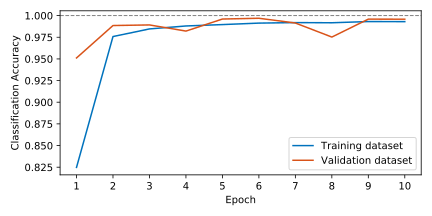
\includegraphics[width=\textwidth]{training_results}
  \caption{Results of the training of the \acrshort{cnn} model}
  \label{fig:training_results}
\end{figure}

\subsection{Saving of the Model}
\label{subsec:training_of_the_cnn:training:saving_of_the_model}
% explain the saving process of the model and the different formats they are saved in .pb / .hdf5 / frozen_graph
% The final model fit is saved in the TensorFlow SavedModel file format (\texttt{saved\_model.pb}).
The final model fit is saved in the TensorFlow SavedModel file format (\texttt{assets/}, \texttt{variables/}, \texttt{saved\_model.pb}), which includes the weights and the computation (e.g. architecture, optimizer state).
% This file format includes the weights and the computation (e.g. architecture, optimizer state), which is useful for sharing and deploying.
This is very useful for sharing and deploying of the \acrshort{cnn} model \cite{training_train_tf_keras_saving_loading}.
% this is a worse citation than the keras one % todo: cite https://www.tensorflow.org/guide/saved_model

% In addition to the 
% Inference tasks commonly use frozen graphs (single \texttt{.pb} file).
Inference tasks commonly use the frozen graph file format (single \texttt{.pb} file), which contains the architecture and the weights.
Xilinx requires such a frozen graph for the quantization of the \acrshort{cnn} model.
% Xilinx requires the model in the frozen graph file format (single \texttt{.pb} file) for .
Unfortunately, TensorFlow dropped support for freezing models since v2.x.
It is, however, still possible to freeze a model created with TensorFlow 2 with the usage of low-level TensorFlow \acrshort{api} calls.
% For this purpose
Listing \ref{lst:frozen_graph} shows how the the \texttt{frozen\_graph.pb} file is created \cite{training_train_frozen}.

For inference tasks, it is important to know the names of the input and output layers of the frozen graph.
How this information can be obtained is shown in listing \ref{lst:frozen_graph} on line \ref{lst:ln:input_info} and \ref{lst:ln:output_info}.
The name of the input layer is \texttt{x} and the name of the output layer is \texttt{Identity}.

\clearpage

\begin{lstlisting}[style=python, caption={Saving the model in the frozen graph file format \cite{training_train_frozen}}, label=lst:frozen_graph]
# Saving the frozen graph
# Convert the Keras model to a concrete function
full_model = tf.function(lambda x: model(x))
full_model = full_model.get_concrete_function(
  x=tf.TensorSpec(model.inputs[0].shape, model.inputs[0].dtype))

# Get the frozen concrete function
frozen_func = convert_variables_to_constants_v2(full_model)
frozen_func.graph.as_graph_def()

# Display information about the input and output layers
print(f'Input: {frozen_func.inputs}')(*\label{lst:ln:input_info}*)
print(f'Output: {frozen_func.outputs}')(*\label{lst:ln:output_info}*)

# Save the frozen graph from the frozen concrete function
tf.io.write_graph(
  graph_or_graph_def=frozen_func.graph,
  logdir=str(fh.dir_frozen_model),
  name='frozen_graph.pb',
  as_text=False)
\end{lstlisting}

